%%%%%%%%%%%%%%%%%%%%%%%%%%%%%%%%%%%%%%%%
%%%%%  xPhO LaTeX Beamer Template  %%%%%
%%%%%  Date: 17/03/2025            %%%%%
%%%%%  Authors:                    %%%%%
%%%%%       Nguyen Thanh Long      %%%%%
%%%%%       Nguyen Le Mai Huong    %%%%%
%%%%%       Nguyen Minh Phuong     %%%%%
%%%%%%%%%%%%%%%%%%%%%%%%%%%%%%%%%%%%%%%%

\documentclass[aspectratio=169, t]{beamer} % Ratio 16:9
\usepackage[T5]{fontenc}
\usepackage{lmodern}
\usepackage{graphicx} 
\usepackage{array}
\usepackage{longtable} % for long table
\usepackage{chngcntr}
\counterwithin{figure}{section}
\usepackage{tcolorbox}
\renewcommand{\familydefault}{\sfdefault} % Font

\usepackage{caption}
\usepackage{siunitx}

\usepackage{tikz}
\usetikzlibrary{patterns}
\usepackage{subcaption}
\let\vec\relax
\newcommand{\vec}[1]{\textbf{#1}}

\usepackage{multicol}

\usepackage{mdframed}

% \definecolor{BlueDefault}{rgb}{0.2,0.2,0.7}
\definecolor{BlueDefault}{RGB}{14,47,95}


% Hide navigation 
\setbeamertemplate{navigation symbols}{}

% Setup background
\newcommand{\normalbackground}{%
    \usebackgroundtemplate{
\includegraphics[width=\paperwidth,height=\paperheight]{Background/Normal_slide_xPhO.pdf}}%
}

\newcommand{\titlebackground}{%
    \usebackgroundtemplate{
\includegraphics[width=\paperwidth,height=\paperheight]{Background/Title_slide_xPhO.pdf}}%
}

% Change the title color to white
\setbeamercolor{frametitle}{fg=white} 

% push the title up by \raisebox
\setbeamertemplate{frametitle}{%
    \vspace{0.3em}
    \hspace{-1em} \insertframetitle
    \vspace{2mm}
}

% Number of slide
\setbeamertemplate{footline}{%
    \hfill
    \insertframenumber/\inserttotalframenumber
    \hspace{7.5mm}
    \vspace{3.5mm}
}

%% Make Table of Contents %%
\AtBeginSection[]{
    \begin{frame}
        \frametitle{Mục lục}
            \tableofcontents[currentsubsection]
    \end{frame}
}

%% Section numbering %%
\setbeamertemplate{section in toc}[sections numbered]
\setbeamertemplate{subsection in toc}[subsections numbered]


\renewcommand{\figurename}{Hình}
\renewcommand{\tablename}{Bảng}

%%%%%%%%%% Pictures drawing %%%%%%%%%%%%%

\usepackage{pgfplots} %%%%%% Regression %%%%
\pgfplotsset{compat = newest}
\usepackage{pgfplotstable}
\usepackage{tikz}
\usepackage{tikz-3dplot} %%%%%% Draw %%%%%%
\usepackage{tikz,tkz-euclide}
\usetikzlibrary{arrows,calc,patterns}
\usetikzlibrary{quotes,angles}
\usetikzlibrary{shapes.geometric}
\usepackage{circuitikz} %%%%% Circuit %%%%
\usetikzlibrary{decorations.pathmorphing,patterns}


%%%%% Bibliography %%%%%
\usepackage[backend=biber,style=ieee]{biblatex}
\addbibresource{citation.bib}

\usepackage{url}
\usepackage{hyperref}
\hypersetup{
	colorlinks=true,
	linkcolor=BlueDefault,
	filecolor=BlueDefault,
    citecolor=BlueDefault,
	urlcolor=BlueDefault,
	pdftitle={Overleaf Example},
	pdfpagemode=FullScreen,
}

%%%%%%%%%% Color setup %%%%%%%%%%%%%

\RequirePackage{xcolor}
\definecolor{wsdred}{HTML}{8E1728}
\definecolor{wsdgrey}{HTML}{75787B}
\renewcommand{\normalcolor}{\color{wsdred}}
\colorlet{ColorOr}{white}

\begin{document}

\titlebackground

\begin{frame}[noframenumbering]
    \thispagestyle{empty}
    \bfseries
    \begin{flushleft}
        \vfill
        \vspace{5mm}
        \textcolor{BlueDefault}{\huge \bfseries Vector và  \\Nhập môn Đại số tuyến tính} \\
        \vspace{8mm}
        \textcolor{black}{\large \bfseries Người trình bày: Carina }
        \vfill
    \end{flushleft}
\end{frame}

\normalbackground

\section{Trường vô hướng và giải tích đa biến}
\subsection{Hàm đa biến}
\begin{frame}
\frametitle{Hàm đa biến}
\begin{figure}
    \centering
    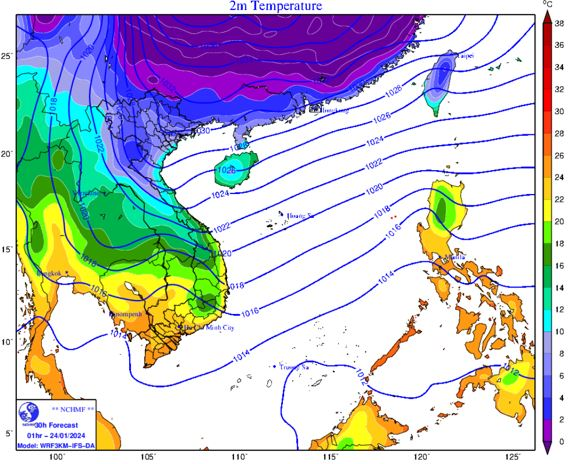
\includegraphics[width=0.5\textwidth]{Content/Figure/TemperatureGraph.jpg}
    \caption{Biểu đồ nhiệt độ theo khu vực}
\end{figure}
\end{frame}

\begin{frame}
\frametitle{Hàm đa biến}
\begin{tcolorbox}[colback=blue!10!, colframe=blue!50!black, title=Định nghĩa]
    Hàm \(f\) theo \(n\) biến là quy tắc gán một véc-tơ \( \mathbf{x} = (x_1, x_2, \ldots, x_n) \) trong tập xác định \(D \subseteq \mathbb{R}^n\) với một số thực \(f(\mathbf{x})\).
\end{tcolorbox}
\begin{figure}
    \centering
    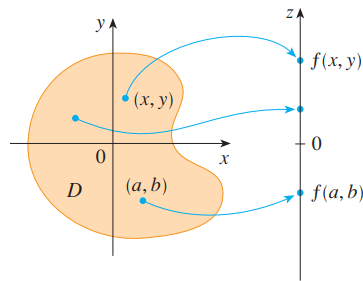
\includegraphics[width=0.3\textwidth]{Content/Figure/MultiVariable.png}
    \caption{Hàm số hai biến \(z = f(x, y)\)}
\end{figure}
\end{frame}

\begin{frame}
\frametitle{Hàm đa biến}
\begin{columns}
\column{0.5\textwidth}
Đồ thị hàm \(f\) bao gồm mọi điểm \((x_1, x_2, \ldots, x_n, z)\) trong \(\mathbb{R}^{n+1}\) sao cho \(z = f(x_1, x_2, \ldots, x_n)\).
\begin{figure}
    \centering
    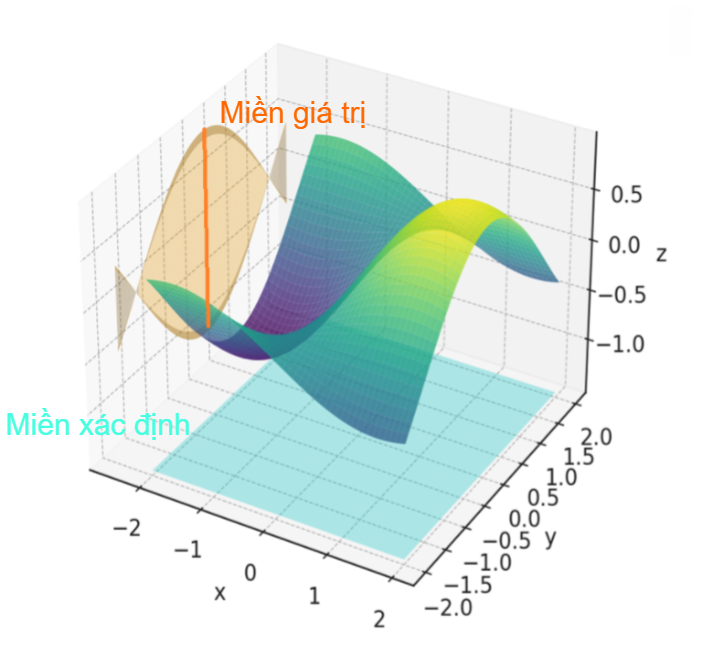
\includegraphics[width=0.65\textwidth]{Content/Figure/Domains.png}
    \caption{Miền giá trị và miền xác định}
\end{figure}
\column{0.5\textwidth}
Một số ví dụ:
\begin{itemize}
    \item \(z=\sin x + \cos y\): \(D = \mathbb{R}^2\), \(z \in [-2, 2]\)
    \item \(z=\sqrt{x+y+1}\): \(D = \{(x,y) | x+y+1 \geq 0\}\), \(z \in [0, +\infty)\)
\end{itemize}
\begin{figure}
\centering
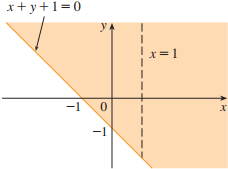
\includegraphics[width=0.5\textwidth]{Content/Figure/MienXacDinh.png}
\caption{Miền xác định của hàm \(z=\sqrt{x+y+1}\)}
\end{figure}
\end{columns}
\end{frame}

\begin{frame}
\frametitle{Hàm đa biến}
Đồ thị đường mức của hàm \(f(\mathbf x)\) là tập hợp véc-tơ \(\mathbf x\) sao cho \(f(\mathbf x)=c\) với một hằng số \(c\).
\begin{columns}
\column{0.5\textwidth}
\begin{figure}
    \centering
    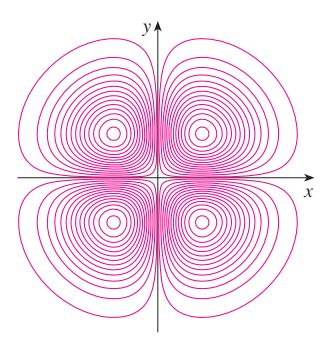
\includegraphics[width=0.53\textwidth]{Content/Figure/contour2d.png}
    \caption{Đường mức của hàm \(z=xy e^{-(x^2+y^2)}\).}
\end{figure}
\column{0.5\textwidth}
\begin{figure}
    \centering
    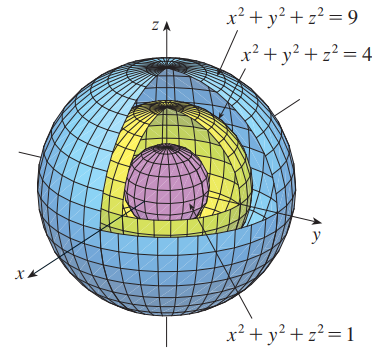
\includegraphics[width=0.61\textwidth]{Content/Figure/contour3d.png}
    \caption{Đường mức của hàm \(f=x^2+y^2+z^2\)}
\end{figure}
\end{columns}
\end{frame}

\subsection{Đạo hàm riêng}
\begin{frame}
\frametitle{Đạo hàm riêng}
\begin{tcolorbox}[colback=blue!10!, colframe=blue!50!black, title=Định nghĩa]
Đạo hàm riêng của hàm \(f(\mathbf x)\) theo \(x_i\) tại điểm \(\mathbf{a} = (a_1, a_2, \ldots, a_n)\) là giới hạn
\begin{equation}
f_{x_i}=\frac{\partial f}{\partial x_i}(\mathbf{a}) = \lim_{h \to 0} \frac{f(a_1, \ldots, a_{i-1}, a_i + h, a_{i+1}, \ldots, a_n) - f(a_1, a_2, \ldots, a_n)}{h}
\end{equation}
nếu giới hạn này tồn tại.
\end{tcolorbox}
Khi này, vi phân của hàm \(f\) tại điểm \(\mathbf{a}\) có thể được biểu diễn như sau:
\begin{equation}
df = f_{x_1} dx_1 + f_{x_2} dx_2 + \ldots + f_{x_n} dx_n
\end{equation}
\end{frame}

\begin{frame}
\frametitle{Đạo hàm riêng}
Xét đồ thị hàm số \(z(x, y)\). Mặt phẳng \(x=a\) và \(y=b\) cắt đồ thị tại hai đường cong \(C_2\) và \(C_1\). Khi đó các đạo hàm riêng chính là độ dốc của các tiếp tuyến \(T_2\) và \(T_1\) của hai đường cong tại điểm \(P(a, b, c)\).
\begin{figure}
    \centering
    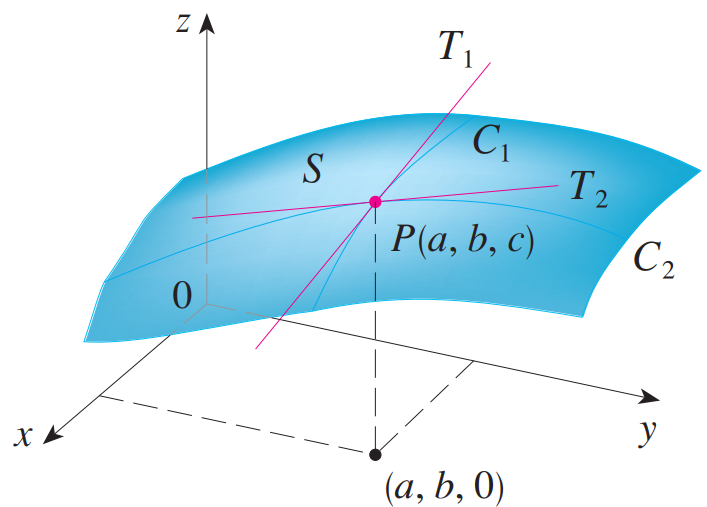
\includegraphics[width=0.4\textwidth]{Content/Figure/PartialDerivatives.png}
    \caption{Ý nghĩa hình học của đạo hàm riêng}
\end{figure}
\end{frame}

\begin{frame}
\frametitle{Đạo hàm riêng}
\begin{tcolorbox}[colback=blue!10!, colframe=blue!50!black, title=Định lý Clairut]
Nếu hàm \(f(x,y)\) có đạo hàm riêng bậc nhất liên tục lân cận điểm \((a,b)\) thì
\begin{equation}
f_{xy}(a,b) = f_{yx}(a,b)
\end{equation}
\end{tcolorbox}
\small
Định lý trên thường được sử dụng trong nhiệt động lực học. Ví dụ, ta có các hàm \(F(T, V)\), \(P(T, V)\), \(S(T, V)\) có các vi phân liên hệ với nhau: \(dF=-SdT-PdV\).

Áp dụng định lý Clairut:
\begin{equation}
F_{TV} = F_{VT} \Rightarrow \left(\frac{\partial S}{\partial V}\right)_T = \left(\frac{\partial P}{\partial T}\right)_V
\end{equation}
Phương trình trên là một trong các phương trình Maxwell trong nhiệt động lực học.
\normalsize
\end{frame}

\subsection{Gradient}
\begin{frame}
\frametitle{Gradient}
\begin{tcolorbox} [colback=blue!10!, colframe=blue!50!black, title=Định nghĩa]
    \textbf{Trường vô hướng} gán tương ứng một giá trị vô hướng cho mọi điểm trong không gian.
\end{tcolorbox}
Ví dụ:
\begin{itemize}
\item Trong bản đồ nhiệt độ, nhiệt độ \(T(\varphi, \lambda)\) được gán với các kinh độ và vĩ độ.
\item Trong trường điện từ, điện thế \(V(x, y, z)\) được gán với các tọa độ trong không gian.
\end{itemize}
\end{frame}

\begin{frame}
\frametitle{Gradient}
\begin{tcolorbox} [colback=blue!10!, colframe=blue!50!black, title=Định nghĩa]
    \textbf{Gradient} của trường vô hướng \(f(x, y, z)\) là véc-tơ
    \begin{equation}
    \nabla f = f_x \mathbf{\hat{x}}+f_y \mathbf{\hat{y}} + f_z \mathbf{\hat{z}}
    \end{equation}
\end{tcolorbox}
Như vậy, ta có thể viết tìm biến thiên \(df\) của hàm \(f\) khi dịch chuyển một đoạn \(d\mathbf r=(dx, dy, dz)\) trong không gian như sau:
\begin{equation}
df = f_x dx + f_y dy + f_z dz = \nabla f \cdot d\mathbf r
\end{equation}
\end{frame}

\begin{frame}
\frametitle{Gradient}
Về mặt hình học, gradient \(\nabla f\) chỉ hướng tăng nhanh nhất của hàm \(f\) và có độ lớn bằng độ dốc theo hướng này.
\begin{figure}
    \centering
    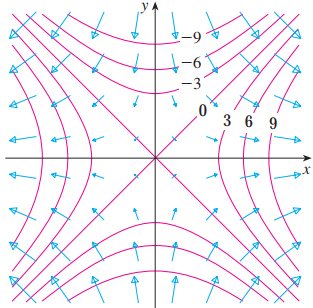
\includegraphics[width=0.3\textwidth]{Content/Figure/gradient.png}
    \caption{Ý nghĩa hình học của gradient}
\end{figure}
\end{frame}

\subsection{Tích phân đa biến}
\begin{frame}
\frametitle{Tích phân bội}
Làm thế nào để tính thể tích của một paraboloid \(z=x^2+y^2\) nằm dưới mặt phẳng \(z=a\)?
\begin{figure}
    \centering
    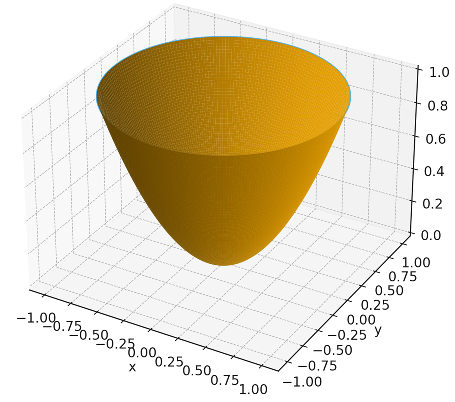
\includegraphics[width=0.4\textwidth]{Content/Figure/paraboloid.png}
    \caption{Paraboloid}
\end{figure}
\end{frame}

\begin{frame}
\frametitle{Tích phân bội}
\begin{columns}
    \column{0.5\textwidth}
    Thể tích \(V\) của paraboloid có thể được tính bằng tổng thể tích của các đĩa dày \(dz\):
    \begin{figure}
        \centering
        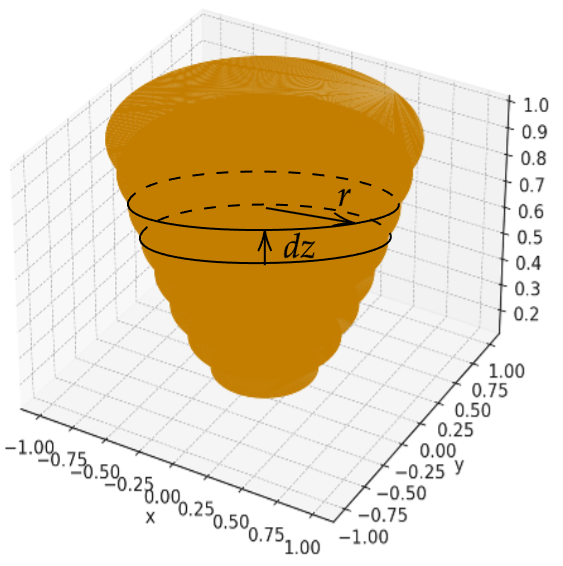
\includegraphics[width=0.7\textwidth]{Content/Figure/discs.png}
    \end{figure}
    \column{0.5\textwidth}
    Trong hệ tọa độ trụ, diện tích của mỗi đĩa được tính bằng tổng diện tích các tam giác nhỏ có góc nhọn \(d\phi\):
    \begin{figure}
        \centering
        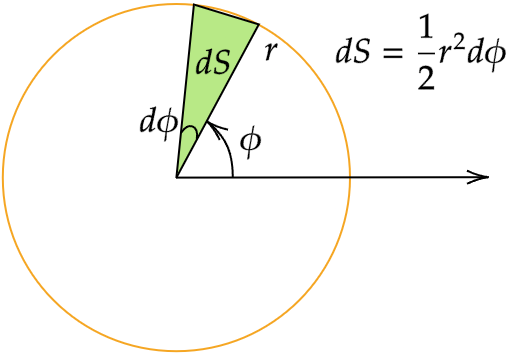
\includegraphics[width=0.8\textwidth]{Content/Figure/cylindricaldisc.png}
    \end{figure}
\end{columns}
\end{frame}

\begin{frame}
\frametitle{Tích phân bội}
Khi đó, thể tích \(V\) có thể được tính như sau:
\begin{equation}
    V= \int_0^a \int_0^{2\pi} \dfrac{r^2}{2} d\phi dz
\end{equation}
Biểu thức trên là một \textbf{tích phân hai lớp}.

Như vậy, thể tích của paraboloid là:
\begin{equation}
    \begin{aligned}
    V&= \int_0^a \pi r^2 dz\\
    &= \int_0^a \pi z dz = \boxed{\dfrac{\pi a^2}{2}}
    \end{aligned}
\end{equation}
\end{frame}

\begin{frame}
\frametitle{Tích phân bội}
\begin{columns}
\column{0.5\textwidth}
Trong hệ tọa độ Đề-các, diện tích của đĩa được tính bằng tổng diện tích của các hình vuông nhỏ có chiều rộng \(dy\):
\begin{figure}
    \centering
    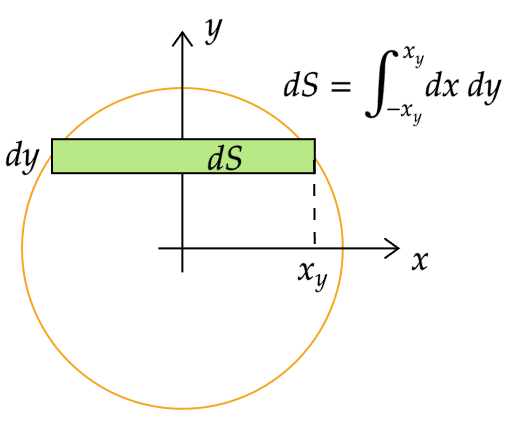
\includegraphics[width=0.7\textwidth]{Content/Figure/descartesdisc.png}
\end{figure}
\column{0.5\textwidth}
Khi đó, thể tích \(V\) có thể được tính như sau:
\begin{equation}
    V= \int_0^a \int_{-\sqrt{z}}^{\sqrt{z}} \int_{-\sqrt{z-y^2}}^{\sqrt{z-y^2}} dx dy dz
\end{equation}
Biểu thức trên là một \textbf{tích phân ba lớp}.

Thực hiện phép tích phân trên, cuối cùng ta vẫn thu được:
\begin{equation}
    V = \boxed{\dfrac{\pi a^2}{2}}
\end{equation}
\end{columns}
\end{frame}

\begin{frame}
\frametitle{Tích phân đường}
Gọi \(\mathbf v(x, y, z)\) là một hàm véc-tơ ứng với mọi điểm trong không gian. \(C\) là một đường cong trong không gian nối hai điểm \(\mathbf a\) và \(\mathbf b\), và có véc-tơ chỉ phương là \(\mathbf u\).
\begin{figure}
    \centering
    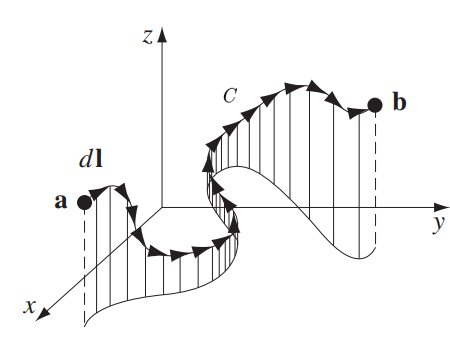
\includegraphics[width=0.3\textwidth]{Content/Figure/tichphanduong.png}
\end{figure}
Khi đó tích phân đường của \(\mathbf v\) dọc theo \(C\) là:
\begin{equation}
\int_C \mathbf v \cdot \mathbf u dl= \int_C \mathbf v \cdot d\mathbf l.
\end{equation}
\end{frame}

\begin{frame}
\frametitle{Tích phân đường}
\begin{tcolorbox}
[colback=blue!10!, colframe=blue!50!black, title=Định lý cơ bản của giải tích]
Nếu \(f\) là một hàm vô hướng có đạo hàm liên tục trong miền chứa đường cong \(C\) nối hai điểm \(\mathbf a\) và \(\mathbf b\), thì
\begin{equation}
\int_C \nabla f \cdot d\mathbf l = f(\mathbf b) - f(\mathbf a).
\end{equation}
\end{tcolorbox}
\end{frame}


\section{Trường vector và giải tích vector}
\begin{frame}
    \frametitle{Trường vector}
    \begin{columns}
        \column{0.5\textwidth}
            \begin{figure}
                \centering
                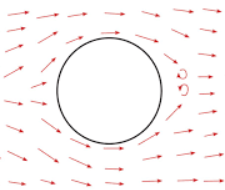
\includegraphics[width=4cm, height=3cm]{Content/Figure/streamline.png}
                \caption{Trường vận tốc của chất lưu}
            \end{figure}
            \[\mathbf{v}=\mathbf{v}(x,y)=\mathbf{v}(r,\theta)\]
        \column{0.5\textwidth}
            \begin{figure}
                \centering
                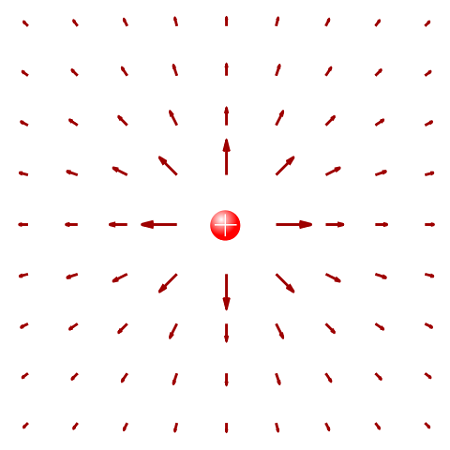
\includegraphics[width=4cm, height=3cm]{Content/Figure/electric_charge.png}
                \caption{Trường tĩnh điện của điện tích điểm}
            \end{figure}
            \[\mathbf{E}=\mathbf{E}(x,y,z)=\mathbf{E}(r)\]
    \end{columns}
\end{frame}
\subsection{Tính xoáy của trường}
\begin{frame}
    \frametitle{Trường (lực) thế}
    \begin{enumerate}
        \item Giá trị của tích phân đường (công) chỉ phụ thuộc vào điểm đầu và điểm cuối: \[-\int_{\mathbf{r}_1}^{\mathbf{r}_2}\mathbf{F}\cdot\text{d}\mathbf{l}=V(\mathbf{r}_1)-V(\mathbf{r}_2).\]
        \item Lưu số trên một đường cong kín là bằng không: \[\oint_{\mathcal{C}}\mathbf{F}\cdot\text{d}\mathbf{l}=0.\]
        \item Trường lực thế có thể biểu diễn dưới dạng gradient của một hàm vô hướng: \[\mathbf{F}=-\nabla V.\]
    \end{enumerate}
    \vspace{-5pt}

    Ví dụ về các lực thế: lực hấp dẫn, lực đàn hồi, \dots
\end{frame}
\begin{frame}
    \frametitle{Quan hệ giữa các tính chất của trường thế}
    \begin{columns}
        \begin{column}{0.5\textwidth}
            \scriptsize
            Từ tính chất thứ nhất,
            \[-\mathbf{F}\cdot\text{d}\mathbf{l}=\text{d}V.\]
            Do đó,
            \[-(F_x \text{d}x +F_y \text{d}y +F_z \text{d}z)=\partial_x V\text{d}x +\partial_y V\text{d}y +\partial_z V\text{d}z.\]
            Đồng nhất hai vế, 
            \[\mathbf{F}=-\nabla V.\]
        \end{column}
        \begin{column}{0.5\textwidth}
            \scriptsize
            Từ tính chất thứ hai (xét trên mặt phẳng \(xy\)),
            \begin{figure}
                \centering
                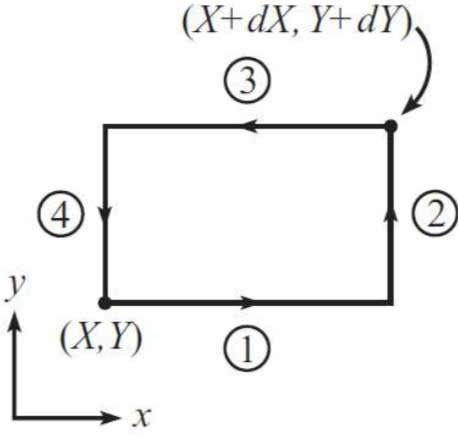
\includegraphics[width=3.5cm, height=3cm]{Content/Figure/Curl.jpg}
            \end{figure}
            \[\oint \mathbf{F}\cdot \text{d}\mathbf{l}=\text{d}X\text{d}Y\left(\partial_x F_y -\partial_y F_x\right)=0.\]
            Tương tự cho các mặt phẳng khác,
            \vspace{-5pt}
            \begin{align*}
                &\text{d}Y\text{d}Z\left(\partial_y F_z -\partial_z F_y\right)=0.&\\
                &\text{d}X\text{d}Z\left(\partial_z F_x -\partial_x F_z\right)=0.&
            \end{align*}
        \end{column}
    \end{columns}
\end{frame}

\begin{frame}
    \frametitle{Curl và định lý Curl (Stokes)}
    \begin{columns}
        \begin{column}{0.5\textwidth}
            \scriptsize
            Curl của \(\mathbf{F}\) được định nghĩa là
            \[\nabla\times\mathbf{F}\equiv \det\left(\begin{bmatrix}
                \hat{x} & \hat{y} & \hat{z}\\
                \partial_x & \partial_y & \partial_z\\
                F_x & F_y & F_z
            \end{bmatrix}\right).\]
            Định lý Stokes tổng quát hoá cho mọi bề mặt:
            \begin{equation*}
                \int_{\mathcal{S}}(\nabla\times\mathbf{F})\cdot\text{d}\mathbf{a}=\oint_{\mathcal{C}}\mathbf{F}\cdot\text{d}\mathbf{l}.
            \end{equation*}
            Chú ý, \(\mathcal{C}\) là đường biên của bề mặt \(\mathcal{S}\). Số hạng ở vế phải được gọi là \emph{lưu số} của trường \(\mathbf{F}\) trên đường cong kín \(\mathcal{C}\).
        \end{column}
        \begin{column}{0.5\textwidth}
            \scriptsize
            Curl của một trường thế bằng không nên \(\mathbf{F}\) phải có dạng \(-\nabla V\) vì
            \[\nabla\times(\nabla V)=0 \quad\forall V.\]
            Cụ thể,
            \begin{align*}
                \partial_{xy}V=&\partial_{yx}V,\\
                \partial_{yz}V=&\partial_{zy}V,\\
                \partial_{zx}V=&\partial_{xz}V.   
            \end{align*}
            Tóm lại, điều kiện cần và đủ của một trường thế là \[\nabla\times \mathbf{F}=\mathbf{0}.\]
        \end{column}
    \end{columns}
\end{frame}
\begin{frame}
    \frametitle{Minh hoạ cho dòng chảy xoáy}
    \begin{columns}
        \begin{column}{0.5\textwidth}
            \begin{figure}
                \centering
                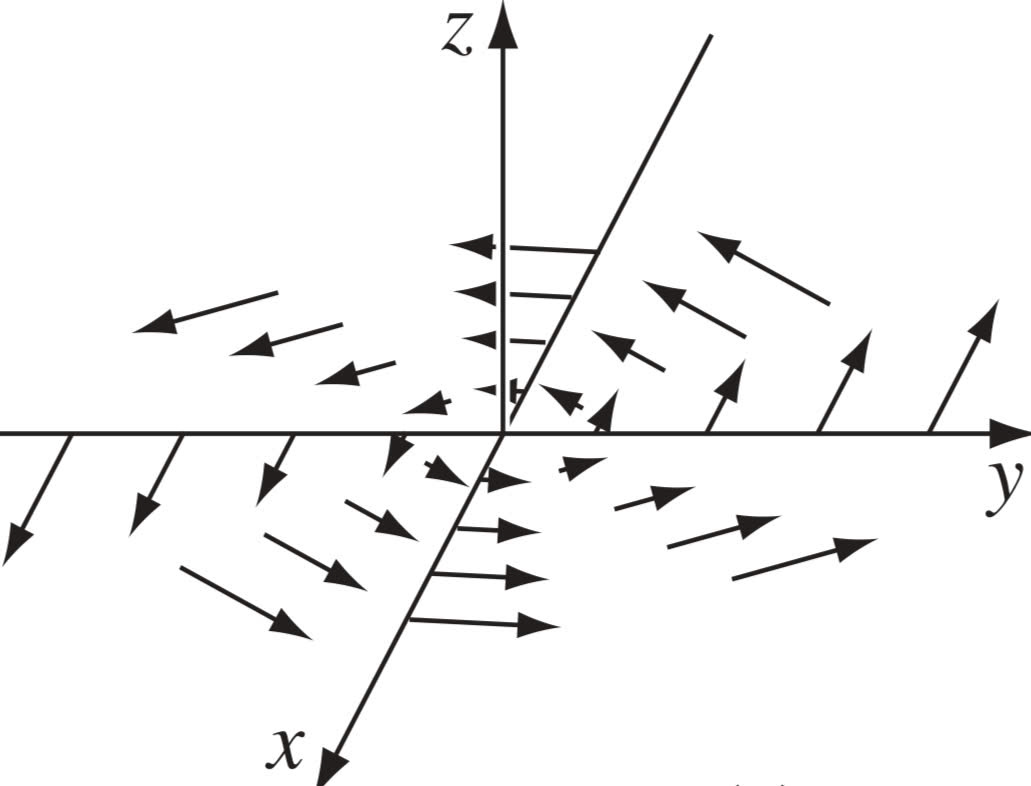
\includegraphics[width=4cm, height=3cm]{Content/Figure/illustration for curl.jpg}
            \end{figure}
            \[\mathbf{v}=-y\hat{x}+x\hat{y},\]
            \[\nabla\times\mathbf{v}=2\hat{z}.\]
        \end{column}
        \begin{column}{0.5\textwidth}
            \begin{figure}
                \centering
                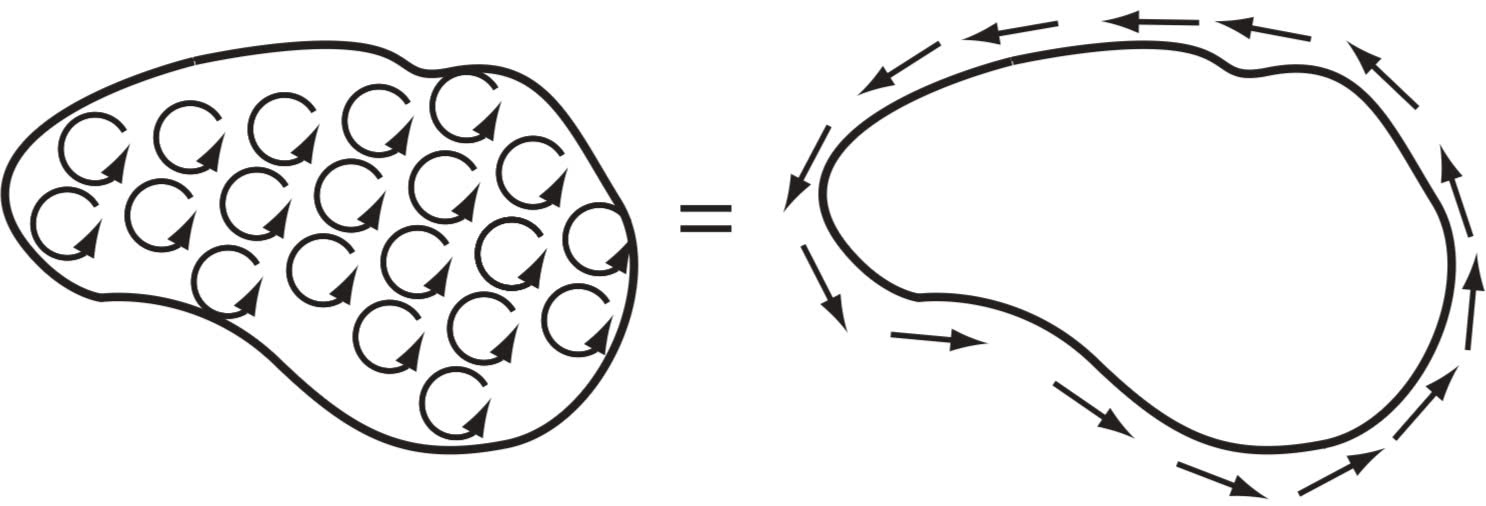
\includegraphics[width=4cm, height=2cm]{Content/Figure/illustration for Stoke.jpg}
                \caption{Định lý Stokes}
            \end{figure}
            \vspace{-8pt}

            \begin{figure}
                \centering
                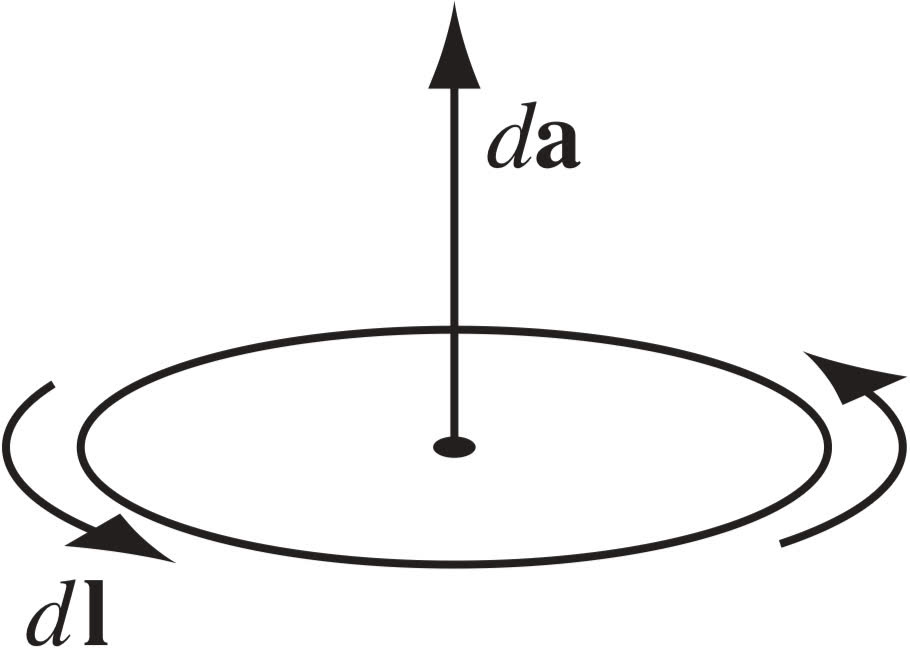
\includegraphics[width=2.5cm, height=2cm]{Content/Figure/direction_of_normal_vector.jpg}
                \caption{Chiều của vector pháp tuyến}
            \end{figure}
        \end{column}
    \end{columns}
\end{frame}
\subsection{Tính phân kỳ của trường}
\begin{frame}
    \frametitle{Thông lượng chất lỏng}
    \begin{figure}
        \centering
        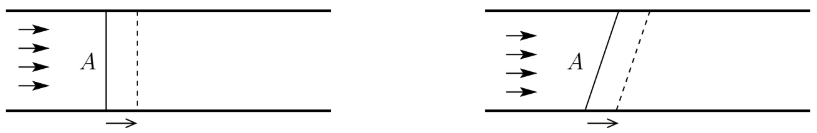
\includegraphics[width=14cm, height=3cm]{Content/Figure/flux of water.png}
    \end{figure}
    \[\text{Lượng nước đi qua tiết diện~}=\mathbf{v}\cdot\hat{n}A\Delta t.\]
    \[\text{Nếu tiết diện gấp khúc: }\sum_{i}^{n}\mathbf{v}\cdot \hat{n}_i A_i \Delta t.\]
    \vspace{-9pt}
    \[\text{Nếu tiết diện là một mặt cong liên tục: } \lim_{n\to\infty}\sum_{i}^{n}\mathbf{v}\cdot\hat{n}_i A_i \Delta t.\]
\end{frame}
\begin{frame}
    \frametitle{Tích phân mặt và thông lượng}
    \begin{figure}
        \centering
        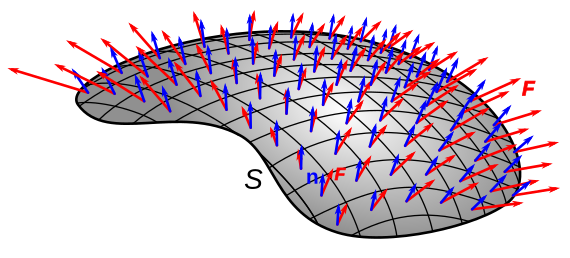
\includegraphics[width=8cm, height=4cm]{Content/Figure/curve_surface.png}
    \end{figure}
    \[\phi=\int_{\mathcal{S}}\mathbf{F}\cdot\text{d}\mathbf{a}.\]
    \(\phi\) được gọi là \emph{thông lượng} của trường \(\mathbf{F}\) qua bề mặt \(\mathcal{S}\).
\end{frame}
\begin{frame}
    \frametitle{Div và định lý Divergence (Gauss)}
    \begin{columns}
        \begin{column}{0.6\textwidth}
            \begin{figure}
                \centering
                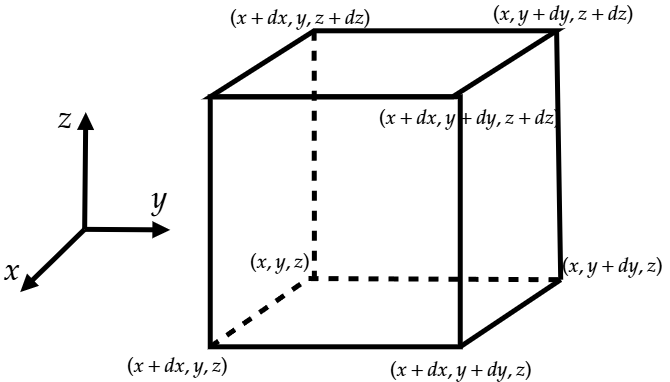
\includegraphics[width=8cm, height=5cm]{Content/Figure/infinitesimal_cube.png}
            \end{figure}
        \end{column}
        \begin{column}{0.4\textwidth}
            \scriptsize
            \begin{align*}
                \delta\phi=& (F_{x}(x+dx)-F_{x}(x))dydz \\
                          +& (F_{y}(y+dy)-F_{y}(y))dxdz \\ 
                          +& (F_{z}(z+dz)-F_{z}(z))dxdy\\
                          =& (\partial_x F_x +\partial_y F_y +\partial_z F_z)dxdydz.
            \end{align*}
            Với \(\nabla\cdot\mathbf{F}\equiv \partial_x F_x +\partial_y F_y +\partial_z F_z ,\)
            \[\delta\phi=\nabla\cdot \mathbf{F}\text{d}\tau.\]
            Định lý Divergence phát biểu rằng
            \begin{align*}
                \oint_{\mathcal{S}}\mathbf{F}\cdot \text{d}\mathbf{a}=\int_{\mathcal{V}}\nabla\cdot\mathbf{F}\text{d}\tau.
            \end{align*}
            
        \end{column}
    \end{columns}
\end{frame}
\begin{frame}
    \frametitle{Nguồn và giếng, phương trình liên tục}
    \begin{figure}
        \centering
        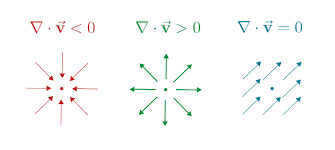
\includegraphics[width=6cm, height=3cm]{Content/Figure/sourrce_fluid.png}
    \end{figure}
    \[\oint_{\mathcal{S}}\mathbf{j}\cdot\text{d}\mathbf{a}+\frac{\partial }{\partial t}\int_{\mathcal{V}}\rho \text{d}\tau =0.\]
    \[\nabla\cdot\mathbf{j}=-\frac{\partial \rho}{\partial t}.\]
\end{frame}
\begin{frame}
    \frametitle{Hình ảnh ví dụ cho một trường vector với các xoáy, nguồn, và giếng}
    \begin{figure}
        \centering
        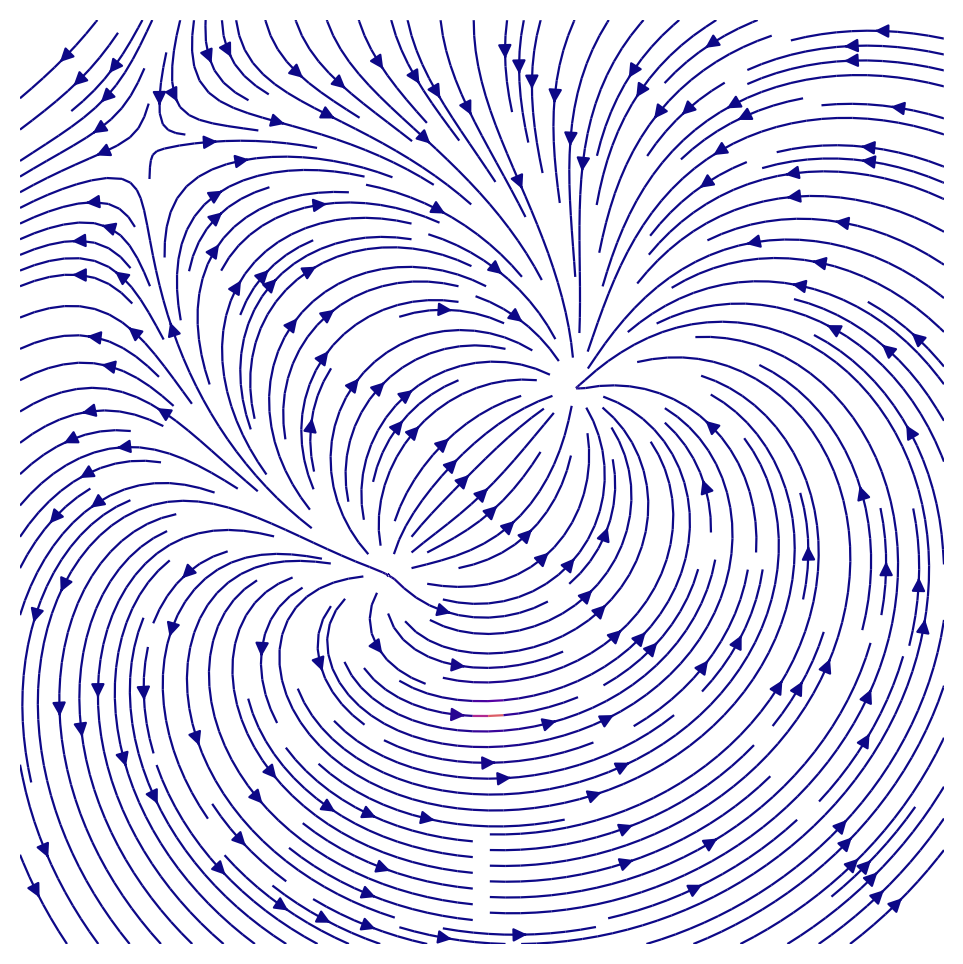
\includegraphics[width=9cm, height=6cm]{Content/Figure/vector_field_expressed.jpg}
    \end{figure}
\end{frame}
\begin{frame}
    \frametitle{Các đạo hàm}
    \begin{enumerate}
        \item \(\nabla\times(\nabla V)=0\) với mọi hàm vô hướng \(V\).
        \item \(\nabla\cdot(\nabla\times \mathbf{F})=0\) với mọi hàm vector \(\mathbf{F}\).
        \item \(\nabla\times(\nabla\times \mathbf{F})=\nabla(\nabla\cdot \mathbf{F})-\nabla^2 \mathbf{F}\), với \(\nabla^2\) là toán tử Laplace, được định nghĩa 
        \[\nabla^2 \equiv \partial^{2}_x +\partial^{2}_{y}+\partial^{2}_{z}.\]
    \end{enumerate}
    Ta cũng có thể viết \[\nabla^2 \mathbf{F}=(\nabla\cdot\nabla)\mathbf{F}.\]
    \scriptsize
    Ngoài ra, \[(\mathbf{u}\cdot\nabla)\mathbf{F}\] biểu thị xấp xỉ tuyến tính cho "vi phân" của \(\mathbf{F}\):
    \vspace{-5pt}
     \[\mathbf{F}(\mathbf{r}+\mathbf{u})-\mathbf{F}(\mathbf{r})\approx (\mathbf{u}\cdot\nabla)\mathbf{F}.\]
\end{frame}
\subsection{Một số ứng dụng}
\begin{frame}
    \frametitle{Áp suất-phương trình cân bằng thuỷ tĩnh}
    Một hệ quả quan trọng của định lý Divergence, với một vô hướng \(T\), là 
    \[\int_{\mathcal{V}}(\nabla T)\text{d}\tau =\oint_{\mathcal{S}}T\text{d}\mathbf{a}.\]
    Với áp suất \(p\) trong chất lỏng, phương trình thu được là 
    \[\int_{\mathcal{V}}(\nabla p)\text{d}\tau =\oint_{\mathcal{S}}p\text{d}\mathbf{a}.\]
    Như vậy, \[-\nabla p +\mathbf{f}_V =\mathbf{0},\] với \(\mathbf{f}_V\) là lực thể tích.
    Trong trường trường hợp của trọng trường,
    \vspace{-5pt}
    \[\nabla p=\rho \mathbf{g}.\]
\end{frame}
\begin{frame}
    \frametitle{Lực hấp dẫn của một khối/vỏ cầu đồng nhất}
    \begin{columns}
        \begin{column}{0.5\textwidth}
            \vspace{-5pt}

             \begin{figure}
        \centering
        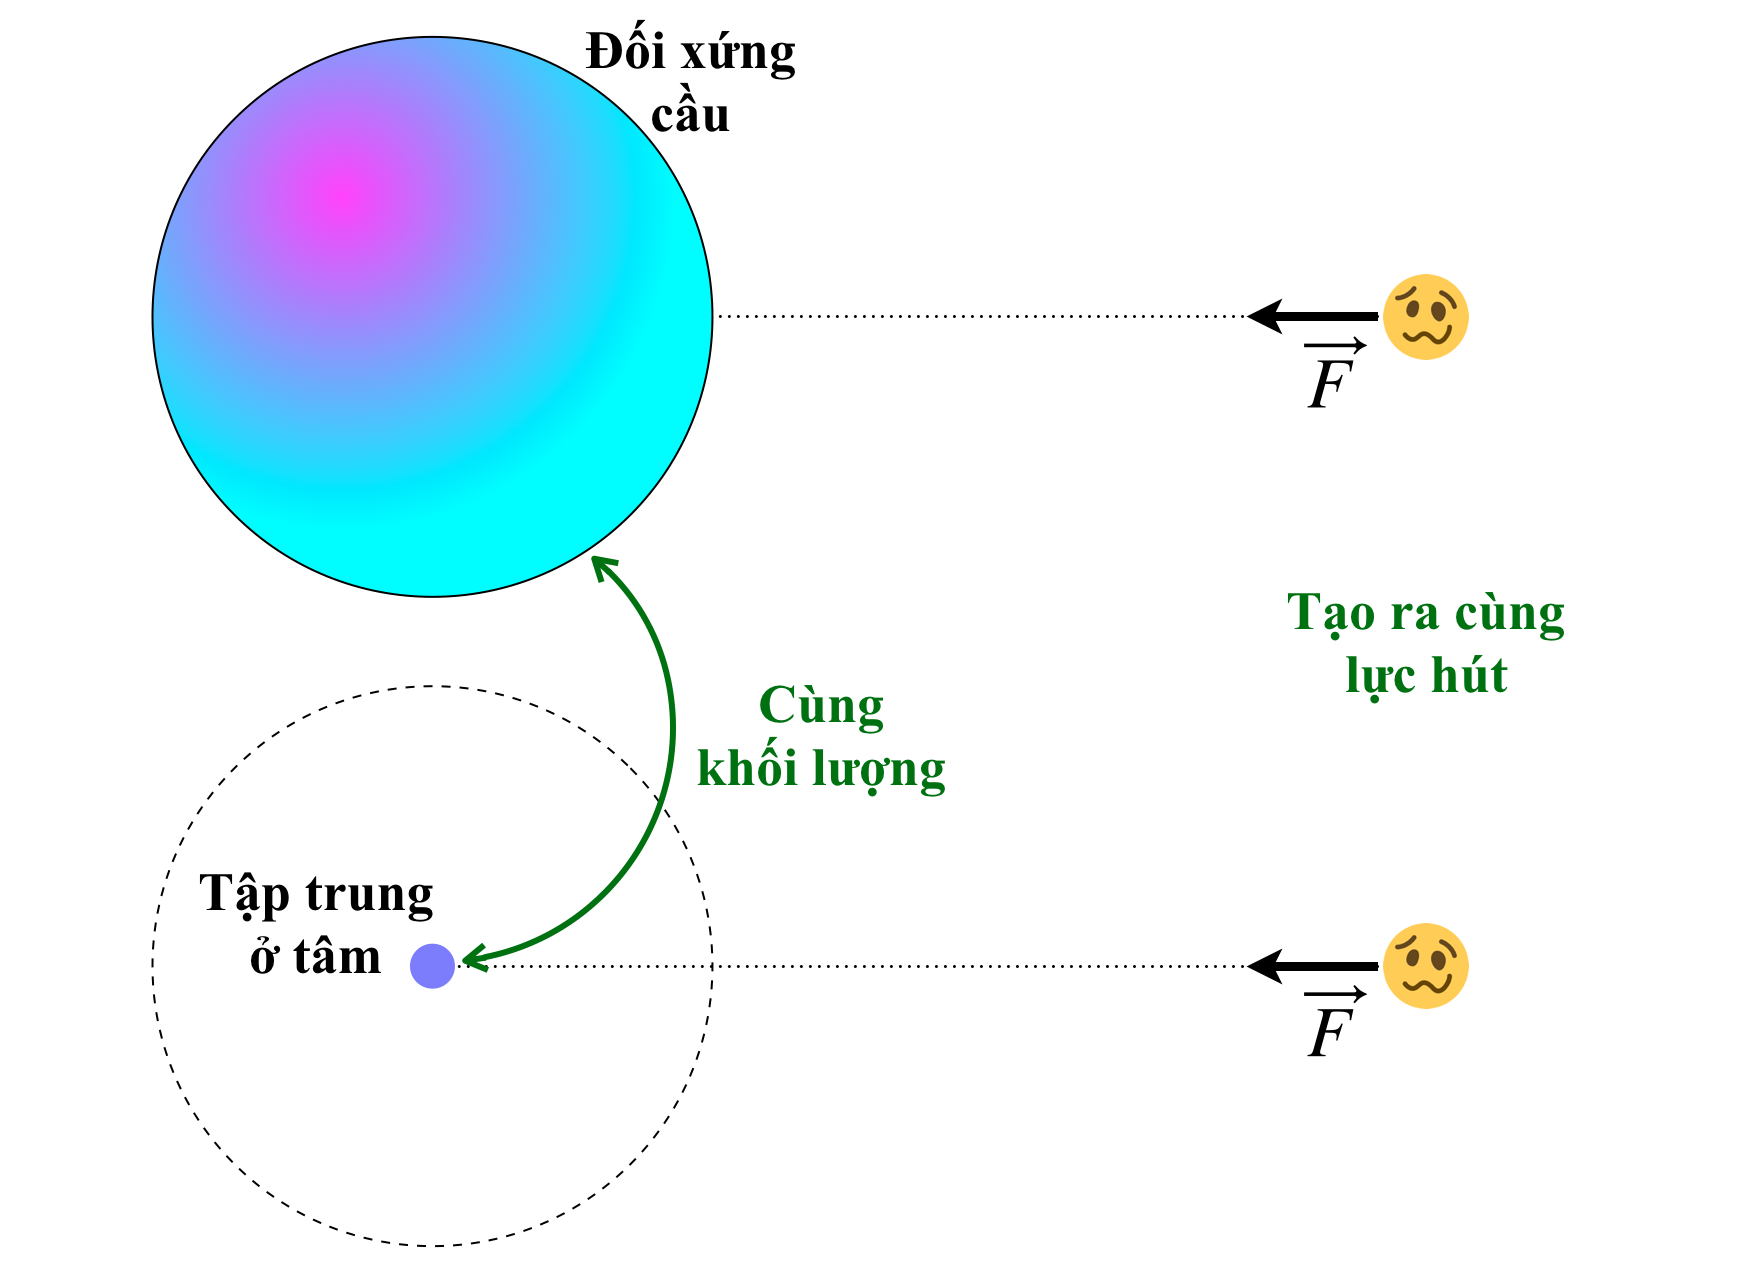
\includegraphics[width=7cm, height=5cm]{Content/Figure/gravity.png}
    \end{figure}
        \end{column}
        \begin{column}{0.5\textwidth}
            \scriptsize
            \[\nabla\cdot\mathbf{F}=\frac{1}{r^2}\partial_r(r^2 F_r)=-4\pi G \rho.\]
           \[\implies (\mathbf{F}\cdot\hat{r})\oint_{\mathcal{S}}da =-4\pi G \rho\times \frac{4\pi}{3}R^3.\]
           \[\implies F_r =-\frac{4\pi G\rho}{3} \frac{R^3}{r^2}.\]
           \[\implies F_r =-\frac{GM}{r^2}\]
            Với \(M=\frac{4\pi R^3}{3}\rho\). Ở đây ta đã đặt \(m=1 kg\).
   \end{column}
    \end{columns}
\end{frame}
\begin{frame}
    \frametitle{Bốn phương trình Maxwell trong chân không}
    \begin{enumerate}
        \item  Định lý Gauss \[\nabla\cdot\mathbf{E}=\varepsilon_{0}^{-1}\rho .\]
        \item  Định lý về sự không tồn tại của đơn cực từ \[\nabla\cdot\mathbf{B}=0.\]
        \item  Định luật Faraday\[\nabla\times\mathbf{E}=-\partial_t \mathbf{B}.\]
        \item Định lý Ampere-Maxwell \[\nabla\times\mathbf{B}=\mu_0 \mathbf{J}+\mu_0\epsilon_0 \partial_t \mathbf{E}.\] 
    \end{enumerate}
\end{frame}
\begin{frame}
    \frametitle{Điện trường của điện tích điểm }
    \begin{columns}
        \begin{column}{0.3\textwidth}
            \begin{figure}
                \centering
                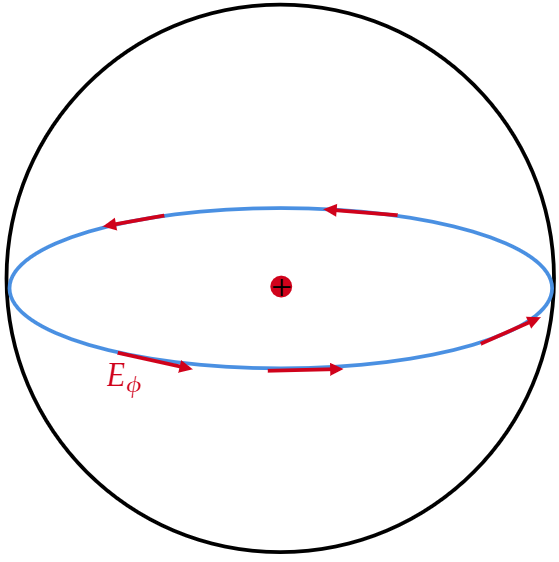
\includegraphics[width=3.5cm, height=3.5cm]{Content/Figure/azimuthal_field.png}
            \end{figure}
            \[E_{\phi}2\pi r =0.\] \[\implies E_{\phi}=0.\]
        \end{column}
        \begin{column}{0.3\textwidth}
            \begin{figure}
                \centering
                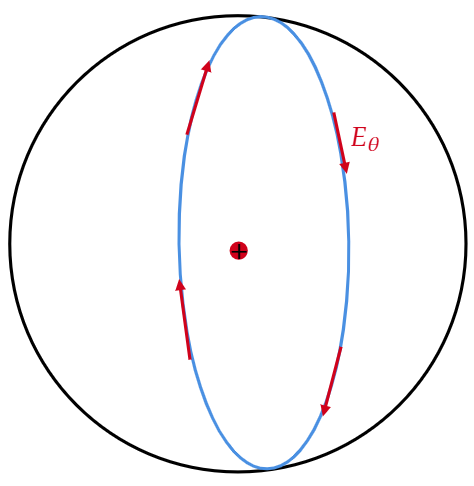
\includegraphics[width=3.5cm, height=3.5cm]{Content/Figure/theta_field.png}
            \end{figure}
            \[E_{\theta}2\pi r =0.\] \[\implies E_{\theta}=0.\]
        \end{column}
        \begin{column}{0.3\textwidth}
            \scriptsize
            Trong tĩnh điện, \(\nabla\times\mathbf{E}=\mathbf{0}\). Thành thử, \[\oint_{\mathcal{C}}\mathbf{E}\cdot\text{d}\mathbf{l}=0.\implies \mathbf{E}=\mathbf{E}_r \hat{r}.\]
            Điều kiện biên:\vspace{-5pt} \[\lim_{r\to\infty}\mathbf{E}(r)\to\mathbf{0}.\]
            Định lý Gauss:\vspace{-5pt} \[\oint_{\mathcal{S}}\mathbf{E}\cdot\hat{r}~da =\varepsilon_{0}^{-1}q.\]
            Như vậy, \vspace{-5pt}\[\mathbf{E}=\frac{1}{4\pi\varepsilon_0}\frac{q}{r^2}\hat{r}.\]
        \end{column}
    \end{columns}
\end{frame}


\begin{frame}[allowframebreaks]{Tài liệu tham khảo}
    \begin{refsection}
        \nocite{morin2008introduction,calculusjame, 3b1b,griffiths2023introduction}
         \printbibliography
    \end{refsection}
\end{frame}

\end{document}